\documentclass[a4paper,11pt]{report}

\usepackage[utf8]{inputenc}
\usepackage[italian]{babel}
\usepackage{amsmath}
\usepackage{amsfonts}
\usepackage{xfrac}
\usepackage{hyperref}

\hypersetup{
    colorlinks=false,
    pdfborder={0 0 0},
}

\usepackage{listings}
\usepackage{lstautogobble}

\lstset{basicstyle=\ttfamily,
  mathescape=true,
  escapeinside=||,
  autogobble}
  
\setlength{\parindent}{0pt}

\newcommand{\der}[2]{\frac{\delta #1}{\delta #2}}
\newcommand{\dder}[2]{\frac{\delta^2 #1}{\delta #2^2}}
\newcommand{\dmix}[3]{\frac{\delta^2 #1}{\delta #2 \delta #3}}

\begin{document}

\thispagestyle{empty}

	\begin{center}
	 {\large{\textbf{POLITECNICO DI MILANO}\\
             Corso di Laurea Magistrale di Ingegneria Matematica\\
             Facolt\`a di Ingegneria dei Sistemi\\
             }}
	\end{center}

	\vspace{1cm}
	\begin{figure}[htbp]
	\begin{center}
	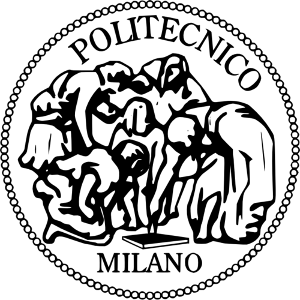
\includegraphics[width=4cm]{img/poli_logo.png}
	\end{center}
	\end{figure}
	
	\vspace{1cm}
	\begin{center}
	{\LARGE{Progetto di Programmazione Avanzata per il Calcolo Scientifico:}}
	\end{center}
	%\color{white}
	\vspace{2cm}
	\begin{center}
	{\LARGE{\textbf{Option Pricing per modelli Exponential-L\`evy in 1d e 2d.}}}
	\end{center}
	
	%\color{black}
	%\vspace{2.5 cm}
	\begin{table}[hb!]
	\begin{center}
	\begin{tabular}{p{8cm}p{7cm}}
	& \\
  	& \\
  	& {\large Nahuel Foresta, matr. 798775}\\
	& {\large Giorgio G. Re, matr. 799260}\\
	\end{tabular}
	\end{center}
	\end{table}
	\begin{center}
	\vspace{3cm}
	\large{Anno Accademico 2012-2013}
	\end{center}

	\clearpage
	\thispagestyle{empty}
	
	\clearpage


\tableofcontents

\setcounter{secnumdepth}{0}

\chapter*{Introduzione}

\chapter{Modello di Black \& Scholes}



\end{document}
